\section{Durchführung}
\label{sec:durchfuehrung}

Um den Versuch durchzuführen wird eine Kupfer-Röntgenröhre verwendet, die die Röntgenstrahlung aussendet.
Zudem wird ein LiF-Kristall zur Brechung benötigt, sowie ein Geiger-Müller Zähler.
Diese Bauteile sind bereits in einem Röntengerät wie in \autoref{fig:bild3} integriert.

\begin{figure}
    \centering
    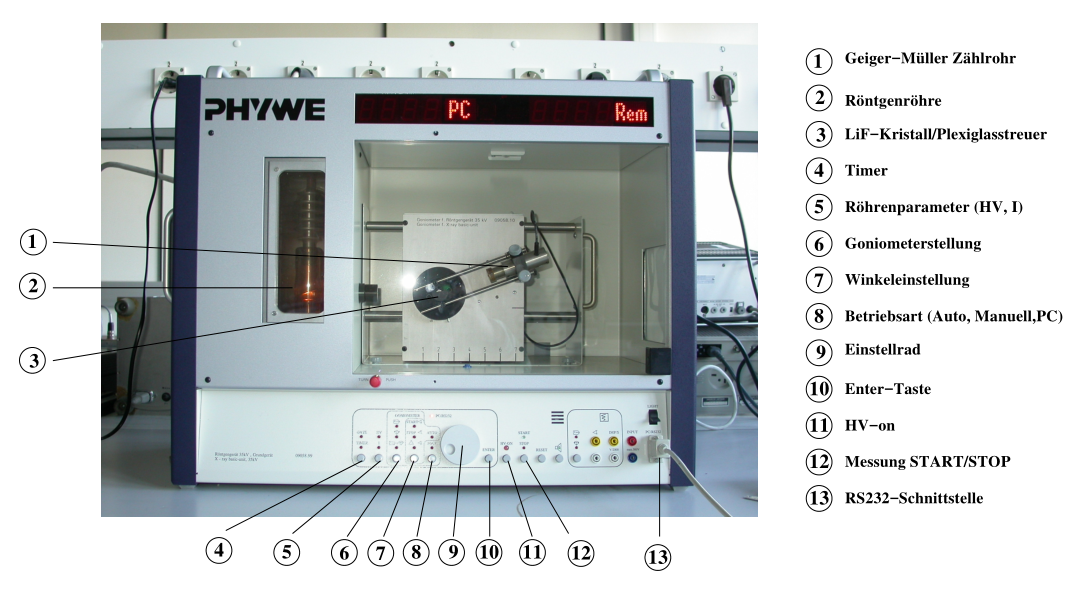
\includegraphics[width=\textwidth/2]{images/bild3.png}
    \caption{Allgemeiner Versuchsbaufbau für die Messungen. \cite{V603}}
    \label{fig:bild3}
\end{figure}

Am Gerät wird eine Beschleunigungsspannung von $\SI{35}{\kilo\volt}$ und ein Emissionsstrom von $\SI{1}{\milli\ampere}$ eingestellt.
Der LiF-Kristall wird in die vorgesehene Halterung gesetzt.

\subsection{Bestimmung des Emissionsspektrums}
\label{ssec:a}

Für diese Messung wird eine $\SI{2}{\milli\meter}$ Blende verwendet.
Der Winkel $\theta$ wird nun auf $\ang{8}$ eingestellt und jede $\ang{10}$ um genau $\ang{0.1}$ verändert.
Diese Messung wird durchgeführt bis der Winkel $\theta = \ang{25}$ erreicht ist.
Alle Winkel und die Ausgaben des Geiger-Müller Zählers werden notiert.

\subsection{Bestimmung der Compton-Wellenlänge}
\label{ssec:b}

Bevor die eigenliche Bestimmung erfolgen kann, wird die Transmission des Aluminiums-Absorbers berechnet.
Dafür wird je eine Messung mit $N_\text{Al}$ und ohne $N_0$ Absorber durchgeführt.
Hier wird der Winkel $\alpha$ von $\ang{7}$ bis $\ang{10}$ in  $\ang{0.1}$ Schritten eingestellt.
Jeder Winkel wird für $\SI{200}{\second}$ beibehalten.
Auch hier werden die Impulse pro Sekunde am Geiger-Müller-Zähler notiert.
Nach der Messung wird eine Totzeit-Korrektur nach \autoref{eq:totzeit} mit $\tau = \SI{90}{\milli\second}$ durchgeführt.

Für die letztendliche Bestimmung der Compton-Wellenlänge wird der LiF-Kristall mit einem Plexiglasstreuer ersetzt.
In drei verschiedenen Messreihen werden nun $I_0$, $I_1$ und $I_2$ berechnet.

$I_0$ kann berechnet werden, indem der Aluminium-Absorber ausgebaut wird und die Intensität der Kupfer-Röntgenröhre unverändert gemessen wird.
Die Impulse werden für $\SI{300}{\second}$ gezählt und dann notiert.

Um $I_1$ zu messen, wird der Absorber zwischen die Röntgenröhre und den Streuer eingebaut, wie in \autoref{fig:bild4} gezeigt wird.
Schließlich werden für $\SI{300}{\second}$ die Impulse gemessen.

\begin{figure}
    \centering
    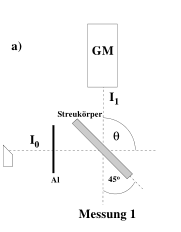
\includegraphics[width=\textwidth/2]{images/bild4.png}
    \caption{Versuchsbaufbau zur Bestimmung von $I_1$. \cite{V603}}
    \label{fig:bild4}
\end{figure}

$I_2$ wird ähnlich wie $I_1$ bestimmt, nur dass der Absorber zwischen Streuer und Geiger-Müller Zähler angebracht wird, der Aufbau ist in \autoref{fig:bild5} dargestellt.
Für $\SI{300}{\second}$ werden wieder die Impulse gezählt.

\begin{figure}
    \centering
    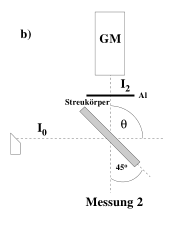
\includegraphics[width=\textwidth/2]{images/bild5.png}
    \caption{Allgemeiner Versuchsbaufbau für die Messungen. \cite{V603}}
    \label{fig:bild5}
\end{figure}